\documentclass{article}
\usepackage[preprint]{neurips_2019}
\usepackage{graphicx,float}
% \usepackage[utf8]{inputenc} % allow utf-8 input
% \usepackage[T1]{fontenc}    % use 8-bit T1 fonts
% \usepackage{hyperref}       % hyperlinks
% \usepackage{url}            % simple URL typesetting
% \usepackage{booktabs}       % professional-quality tables
% \usepackage{amsfonts}       % blackboard math symbols
% \usepackage{nicefrac}       % compact symbols for 1/2, etc.
% \usepackage{microtype}      % microtypography
\title{Predicting Stocks Trends Based on News}
\author{
Harsh Dedhiya, Raghav Malhotra, Phumin Walaipatchara\\
Department of Computer Science\\
Boston University\\
\texttt{hdedhiya@bu.edu, raghav20@bu.edu, phuminw@bu.edu}\\
}
\begin{document}
\maketitle
\begin{abstract}
The stock market is known to show emerging trends in the way of its computation and it is times
 of volatility that spontaneous judgments are needed to be made to speculate price behaviour.
 A platform which trains a predictive model through mining the news for headlines and words
 pertaining demonstrating an ascertainable correlation to share price changes is exemplary to
 the application of AI in finance. With the use of recurrent neural networks that incorporate LSTM,
 logistic regression, naïve bayes, term frequency and a simultaneous focus on political events keeping
 in mind the obsolete tendency. This attributes to the automation dynamic of the pertinent algorithms
 that would be amended to such occurrences.
 \\\\
 An example of this is, the dense implementation of blockchain in financial circulation that would
 give regulation less effective control of the financial industry and its cohorts. By this measure,
 the inability of the federal reserve to intervene in fabric of the stock market (with blockchain,
 monetary policy will not affect share prices). This is one conceptual aspect of several that call for
 existing models and algorithms to be subject to amendments. Cross validations are also performed between
 years and on a continuum to increase precision of the models and optimise them.
\end{abstract}
\section{Dataset}
Some text for second section

\section{Na\"ive Bayes}
Describe the result from Na\"ive Bayes approach

\section{Logistic Regression}
Describe the result from logictic regression

\section{Sentiment Analysis}

\section{Recurrent Neural Network}
\indent In order to capture the objective of accurate prediction, Recurrent Neural Network (RNN) is introduced
 because its ability to exhibit internal state (memory). Specifically, Long short-term memory (LSTM),
 a special kind of RNN, is used for implementation as LSTM can deal with vanishing gradient problems
 and is capable of learning long-term dependencies.
\\
\begin{figure}
    \centering
    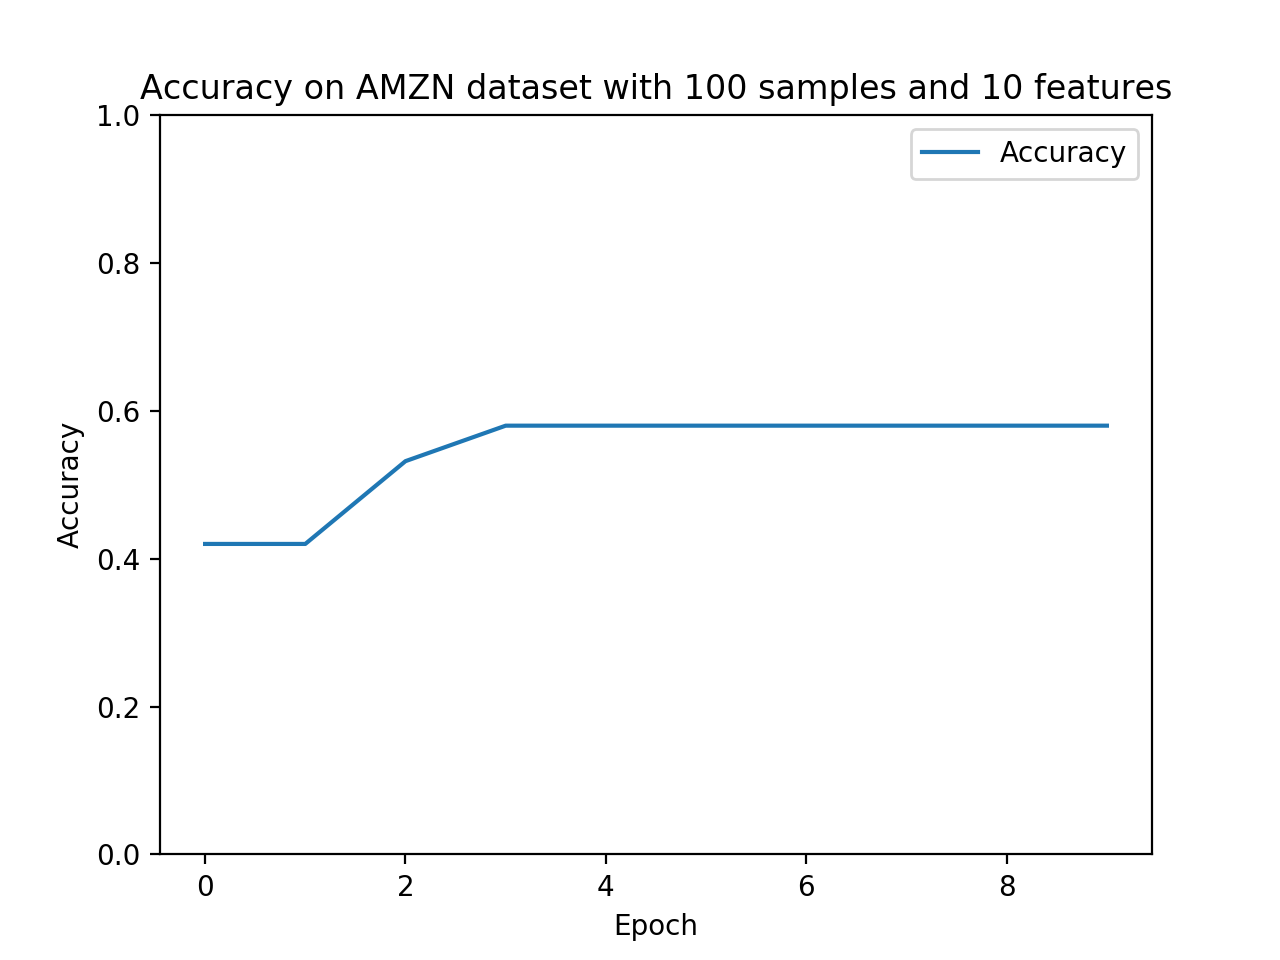
\includegraphics[scale=0.5]{assets/Accuracy.png}\\
    \caption{Accuracy of the model}
\end{figure}
\begin{figure}
    \centering
    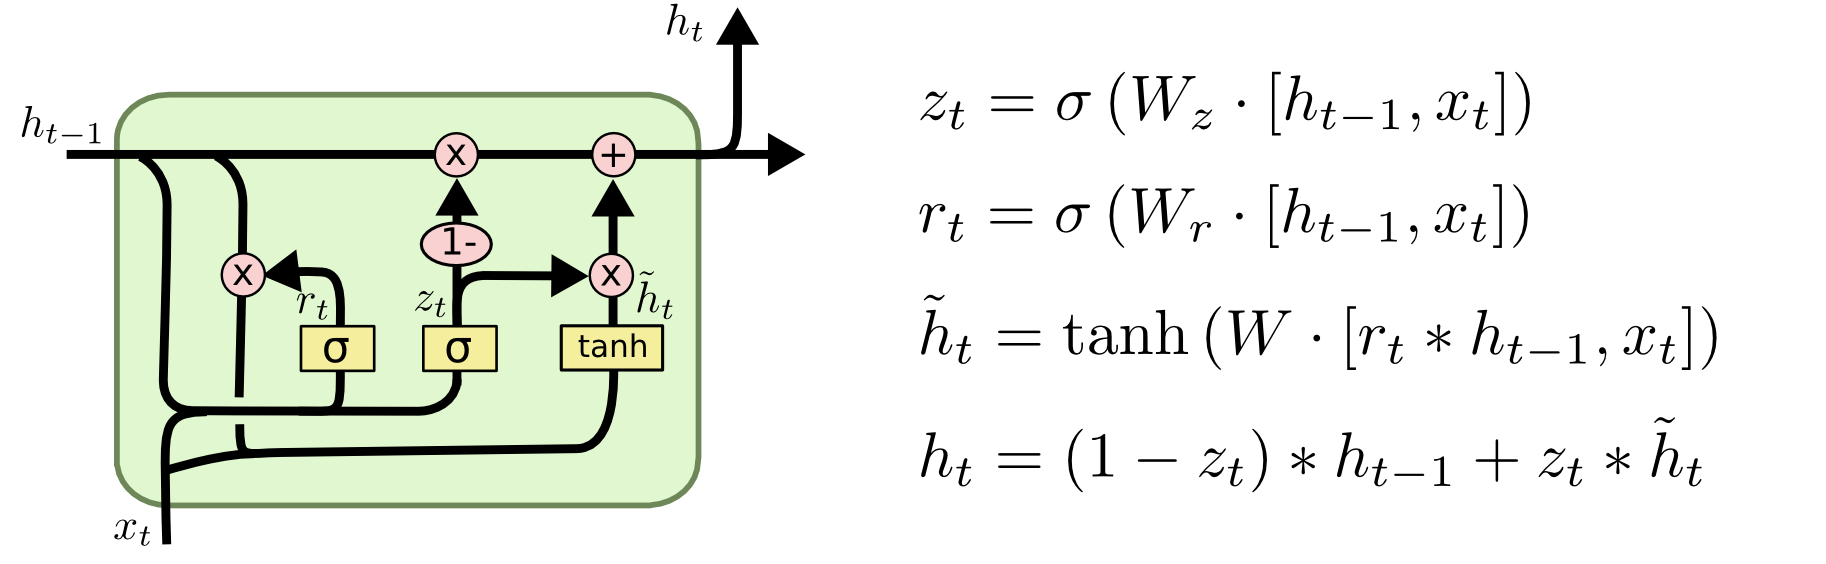
\includegraphics[scale=0.4]{assets/LSTM.png}
    \caption{LSTM structure}
\end{figure}
Before begin training the model, the dataset, 100 samples in this case, must be preprocesed introduced
 boolean vector through $TfidfVectorizer$ from $sklearn.feature\_extraction.text$. The $max_features$, which is
 also the size of the boolean vector is specified to be 10. Each sample (now a boolean vector) is paired up with
 the stock (AMZN in this case) movement, 1 for going up and 0 otherwise. In one epoch, we use $KFold$ from
 $sklearn.model_selection$ to split the dataset into 2 groups, one for training and one for testing.
\\\\
 Regarding network structure, the LSTM network has 10 input nodes, which corresponds to the size of
 the boolean vector. It has 4 hidden nodes between the input layer and the LSTM and use sigmoid as an activation
 function. After LSTM module, the output layer consisting of 2 nodes uses softmax as an activation function in order
 to represent output as a probability of classification.
\\\\
During the training period of the network, the parameters (learning rate, $max_feature$, and number of sample) have
 to be adjusted to some specific configuration in order to show the improvement of training as shown in Figure 1.
 Greater or lesser the value of parameters will result in stationary accuracy since the first epoch, which is not
 useful for parameter tuning process and training process.
\\\\
Currently, the only indicator that was taken into account is news headlines as a boolean vector through $TfidfVectorizer$.
 However, there are more factors that can be used as indicators for prediction, for instance, the unemployment rate,
 volume, social network, interest rate, etc. Those indicators should be fed into the network as well, but they need
 to be processed/weighted appropiately proportional to the importance of each indicator. As described, there are lots
 of rooms for improvement for this network and also for integrating other techniques to improve the accuracy of prediction.
\section*{References}
if needed

\end{document}
